% 设置 biblatex 额外选项
% \PassOptionsToPackage{gbpub=false, gbtype=false}{biblatex}

\documentclass[degree=course, language=chinese]{sjtuthesis}
% 选项
%   degree=[doctor|master|bachelor|course],     % 必选,学位类型
%   language=[chinese|english],                 % 可选(默认:chinese),论文的主要语言
%   bibstyle=[gb7714-2015|gb7714-2015ay|ieee],  % 可选(默认:gb7714-2015),参考文献样式
%   review,                                     % 可选(默认:关闭),盲审模式

% 所有其它可能用到的包都统一放到这里了,可以根据自己的实际添加或者删除。
\usepackage{sjtuthesis}
\usepackage{float}
\usepackage{amsmath}

% 定义图片文件目录与扩展名
\graphicspath{{figure/}}
\DeclareGraphicsExtensions{.pdf,.eps,.png,.jpg,.jpeg}

% 导入参考文献数据库
\addbibresource{bib/thesis.bib}

% 信息录入,必须在导言区进行!
% !TEX root = ../thesis.tex

%TC:ignore

\title{大数据场景下的语言虚拟机优化调研} 
\author{丁贞锴   119037910044}
\studentid{陈一雄   119037910003}
\supervisor{陈悦    119037910017}
\department{齐明   119037930071}


%TC:endignore


% 自定义项目标签名称
% \sjtuSetLabel{
%   listfigure = {图\quad 录},
%   listtable  = {表\quad 录}
% }

\begin{document}

% 无编号内容:中英文论文封面、授权页
\maketitle

% 使用罗马数字对前言编号
\frontmatter

% 摘要
% !TEX root = ../thesis.tex

\begin{abstract}
  大数据时代带来了大数据项目的爆炸式发展。随着各个项目的发展与日益成熟,通过改进分布式计算框架本身来大幅提高性能的机会越来越少。越来越多的开发者将眼光投向了运行大数据框架的高级语言虚拟机本身,
  希望通过解决虚拟机本身的一些问题,提高分布式系统的性能和健壮性。
  由于这些高级语言虚拟机在最初设计时并没有充分考虑到大数据处理应用的特点,因此在性能方面往往会存在问题。近年来,有很多研究者从不同方向尝试解决这些问题。
  本文对大数据场景的研究进行调研,总结高级语言虚拟机存在的问题,具体分析垃圾收集器Yak的研究思路及其局限性,并针对Yak提出优化方案。
\end{abstract}


% 目录、插图目录、表格目录
\tableofcontents
\listoffigures
\listoftables
\listofalgorithms


% 使用阿拉伯数字对正文编号
\mainmatter

% 正文内容
% !TEX root = ../thesis.tex

\chapter{介绍}
过去十年见证了大数据的爆炸式发展,人类社会以前所未有的规模和速度创建大量数据。第二次工业革命以后,数据量越每10年翻一番;
从20世纪50年中期开启的信息革命带来的巨大生产力发展,导致人类社会从工业化时代进入信息化时代,新数据的产生进一步加速,约每三年翻一番。
前谷歌首席执行官埃里克·施密特在Techonomy'10会议上分享,现在短短2天产生的数据量比2003年之前整个人类社会产生的数据总量还多。
据国际数据公司(IDC)发布的2017年大数据白皮书预测,2025年全球大数据规模将增长至163ZB,相当于2016年的10倍。
大量数据的可利用性催生了大规模的数据密集型应用。大数据分析迅速成为一门重要研究,在金融、商业、医疗保健和政府管理等重要领域发挥作用,进而服务整个社会。
例如电商公司和广告公司可以对用户历史数据进行分析,来给用户提供个性化的产品;银行等金融机构的风控部门可以对每天的交易数据进行分析,打击金融诈骗等违法犯罪行为;
政府部门可以分析一段时间的人流数据,决定新的地铁站最合适的位置。

随着数字世界的不断扩展和大数据分析技术在社会生活中日益增长的重要性,公司、政府机构和学术机构对可快速运行大数据分析程序分析大规模数据的可扩展系统的需求也日益增长。
解决可扩展性挑战的主流方法是使用大量计算节点来进行分布式处理。常用的大数据处理系统包括Hadoop、Spark、Hive、DryadLinQ、Flink等。这些大数据处理系统大多是使用Java、
C\#或者Scala等面向对象的托管式语言开发的,因为托管式语言提供了快速开发的特性:自动内存管理和丰富的社区支持。但是使用托管式语言开发的程序必须要运行在托管式语言提供的
运行环境(runtime)或者更具体一点是托管式语言提供的虚拟机上。但是这些语言虚拟机在最初设计时并没有考虑到大数据的特性:TODO大数据特性, 因此大数据分析程序运行时,runtime
会带来巨大的性能开销,例如runtime内存管理中垃圾回收(GC)常常会占用40\% ~ 60\%的执行时间。

TODO 具体描述runtime性能开销

托管式运行时带来的如此大的性能开销是不可以接受的,那我们是不是可以抛弃托管式语言,回到非托管式语言?答案是否定的。使用非托管式语言例如C或C++进行开发确实可以避免托管式语言带来的
内存管理开销,但这也丧失托管式语言带来的便利:快速开发。众所周知,使用非托管式语言进行开发需要自己做内存管理等一系列工作,开发者需要写的代码更多,相应的,出错的概率也就越大。并且,
以非托管式语言调试内存错误是一项很痛苦的任务,尤其是在大数据处理系统数据量大、分布式执行环境和运行时间较长的特性下,调试的工作量更大。同时,由于大多数现有的大数据处理框架已经以
托管式语言进行开发,全部推倒以非托管式语言重构工作量太大,基本是不现实的。

因此,主流的研究方向还是在对现有的托管式runtime,主要是语言虚拟机进行优化。






\chapter{背景}

\section{GC}
GC(垃圾收集)是托管式语言Java、Scala等与非托管式语言像C或C++的主要区别之一。
使用托管式语言进行开发,不需要专门编写内存分配与回收代码,也不需要去考虑
内存泄漏和溢出的问题。这确实给开发人员降低了不少工作压力,但也带来了两个新问题。
其一,GC时间开销太大,成为性能瓶颈,降低可扩展性。其二,由于内存管理都是托管的,
开发人员不能详细了解内存管理情况。这就导致一旦发生内存溢出与内存泄漏问题,开发人员
需要花更多的精力去解决。换言之,由于内存管理是托管的,内存管理的正确性与性能也都由
托管式语言对应的高级语言虚拟机(Java语言的JVM,.Net语言的CLR等)决定。所以一旦虚拟机的
垃圾回收策略与当前运行场景不适配(这常常发生,因为虚拟机的垃圾回收策略相对稳定,
大约2-3年才会更新一次,但是新场景层出不穷,所以往往策略是不能完全适配场景),那么内存管理的性能与正确性都会变得很糟糕。
GC的任务是解决以下三个问题:哪些内存需要回收、什么时候回收和如何回收。

\begin{figure}[h]
    \centering
    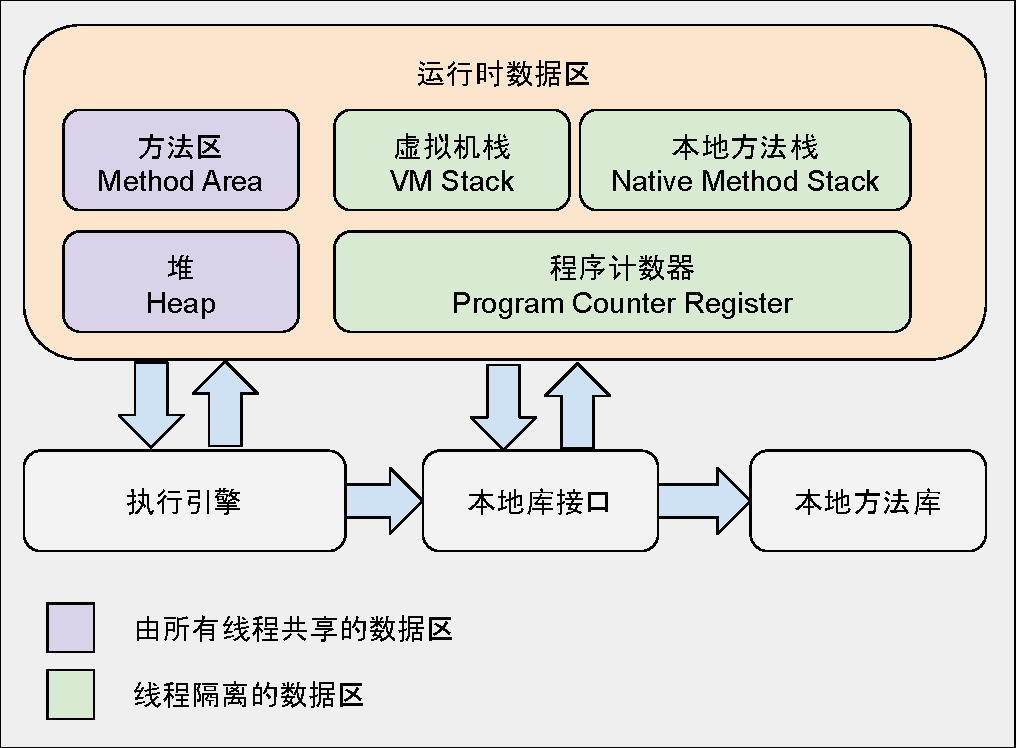
\includegraphics[width=12cm]{figure/JVM_memory_layout.pdf}
    \caption{JVM运行时数据区\cite{Understand_JVM}}
    \label{jvm_memory_layout}
\end{figure}

回答这三个问题首先需要了解虚拟机中的内存布局。以JVM为例,JVM在执行Java程序的过程中会把他所管理的内存划分为弱冠个不同的数据区域。
JVM运行时数据区如图\ref{jvm_memory_layout}所示。程序计数器存储正在执行的虚拟机字节码的地址。虚拟机栈包含局部变量表、操作数栈、动态链接、方法出口等信息。
其中局部变量表所需的内存空间在编译时完成分配,当进入一个方法时,这个方法需要在帧中分配多大的局部空间是完全确定的,不会改。
本地方法栈存储JNI调用。堆在虚拟机启动时创建,此内存区域唯一目的是存放对象实例。所有的对象实例和数据都要在堆上分配,
但是随着JIT编译器的发展与逃逸分析技术逐渐成熟,栈上替换、标量替换将会导致一些微妙的变化。方法区
存储被虚拟机加载的类信息、常量、静态变量、即时编译器编译后的代码等数据。其中方法区和堆是线程共享的,
也是JVM GC所针对的数据区。

哪些内存需要回收?托管式语言虚拟机中,数据是以对象的形式存储在堆中,对象由对象头、实例数据和对齐三部分组成。
其中对象头包含对象自身运行时的数据包括对象的hashcode、GC分代年龄等;实例数据包含对象的属性数据包括以指针形式存在的
指向其他对象的引用。GC主要针对的是堆中未被引用的对象。寻找未被引用对象是通过可达性分析算法实现的。可达性分析算法以
\texttt{GC Root}对象作为起点沿着对象间的引用链向下搜索,搜索不到的对象为不可达对象,GC时会被回收。\texttt{GC Root}
是GC被调用时一定存活的对象,JVM中\texttt{GC Root}由以下四种对象组成:
\begin{enumerate}
    \item 虚拟机栈(栈帧中的本地变量表)中引用的对象
    \item 方法区中类静态属性引用的对象
    \item 方法区中常量引用的对象
    \item 本地方法栈中JNI引用的对象
\end{enumerate}

在内存不够用时,虚拟机会调用GC。那么GC是如何运行的?虚拟机是通过不同的垃圾收集算法来执行GC的。包括标记-清除算法、
标记-整理算法、复制算法、分代收集算法和基于region的分代收集算法。标记-清除算法是指通过可达性分析标记出不可达对象后,直接清除。
标记-清除算法有两个不足:其一,清除之后会产生大量碎片,无法分配大对象;其二标记与清除两个过程都是针对整个堆,比较耗时。
复制算法将可用内存分为大小相等的两块,每次只使用其中一块,当一块内存用完时,将这块内存上还存活的对象复制到另一块内存上去,再将这一块内存全部清理掉。
复制算法解决了大量数据对象需要被清除时,清理耗时的问题,提高了效率,也解决了碎片化的问题。但是可用内存减小了,并且如果存活对象较多,复制也会比较耗时。
标记-整理算法将存活对象向顶端或低端移动,清除边界之外的对象,解决了标记-清除算法的碎片化问题,也较为高效,并且相对于复制算法,
标记-整理算法使用了全部的内存。

标记-清除算法、标记-整理算法和复制算法都是对整个堆进行标记和移动,当对象分配的越来越多时,标记和移动也越来越耗时。
但是,根据对Java应用的分析,数据对象的生命周期是不一样的。大部分对象的生命周期很短,小部分对象的生命周期很长。
分代收集算法就是基于这种观察结果被提出的。
分代收集算法将数据对象根据生命周期的不同分为新生代和老生代,并且将堆空间分为几块用来存放不同生命周期的对象,
分别应用最合适的垃圾收集算法。新生代生命周期较短,GC过后只有少量存活,所以使用复制算法。老生到对象存活率较高,
使用标记-清除或者标记-整理算法。对象被创建时,大对象直接进入老生代,小对象就在新生代进行分配,多次GC后任然
存活的对象会进入老生代。一般老生代会占据60\%以上的堆空间。显然新生代相较于老生代GC会比较频繁,新生代GC也只要对
新生代的做可达性分析,然后使用复制算法,老生代GC次数较少。因此分代收集算法提供了最高的收集效率。

\begin{figure}[h]
    \centering
    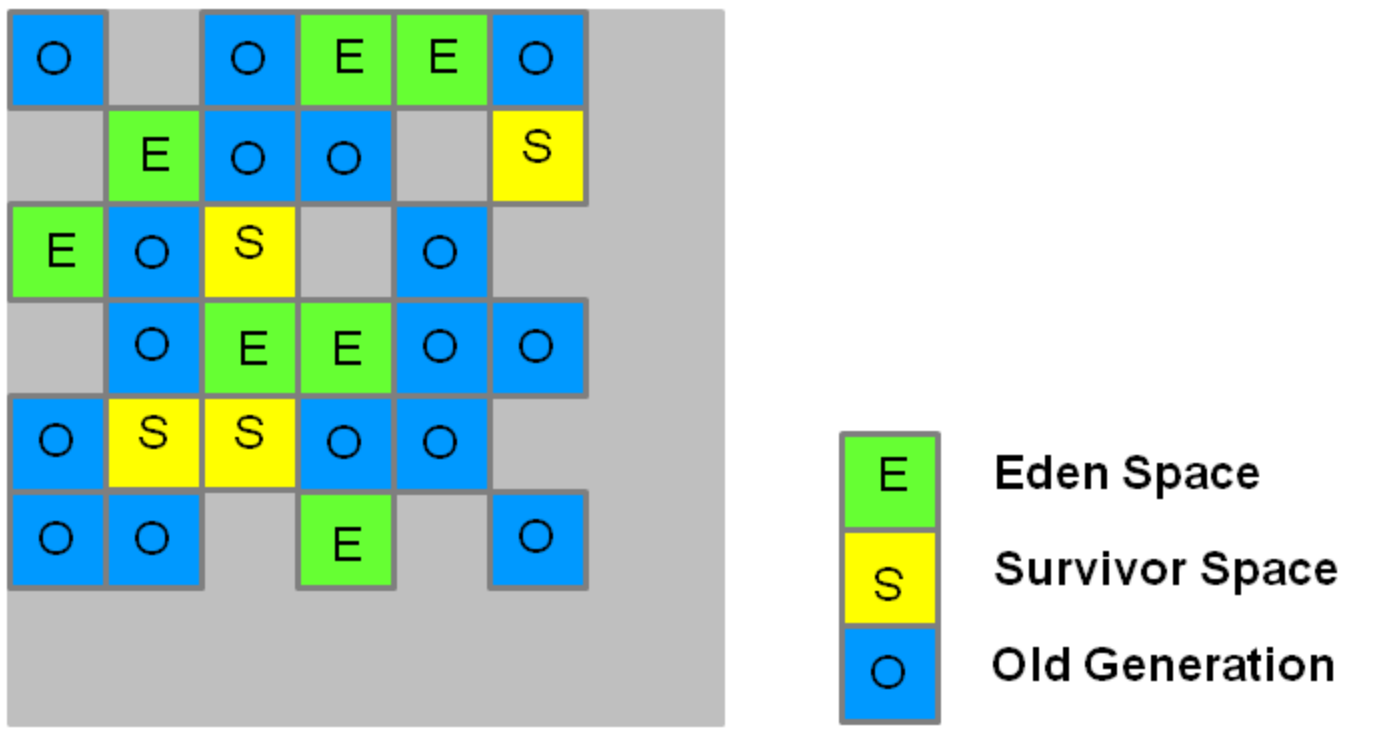
\includegraphics[width=12cm]{figure/region-based-gc.png}
    \caption{基于region的分代收集算法堆空间布局\cite{G1}}
    \label{jvm_region-gc}
\end{figure}
在相同条件下, 堆空间越大, 一次GC耗时就越长, 从而产生的停顿也越长。分代收集算法将堆空间划分为新生代与老生代两部分,
相较于之前,极大提高了效率。但是GC开销还是过大,现代服务器要求每次GC的时间要尽量短,最好控制在某个上限之下。因此
基于region的分代收集算法(又名分区分代收集算法)应运而生。如图\ref{jvm_region-gc}为了更好地控制GC产生的停顿时间, 基于region的分代收集算法将一块大的内存区域分割为多个小块, 
根据目标停顿时间, 每次合理地回收若干个小区间(而不是整个堆), 从而减少一次GC所产生的停顿。基于region的分代收集算法是目前
最新的垃圾收集算法,其性能也最忧。

大数据场景中,数据对象可以按控制路径与数据路径分为用于分布式节点调度的对象和用于装载数据、计算并表示结果的对象。
控制路径对象的生命周期符合新生代老生代的分代特征,使用分代收集算法即可。但是数据路径对象生命周期不符合分代特征。
它们的生命周期呈现出与完全不同的epoch特性,不适合传统GC。epoch特性是指一组对象在同一时间被创建,
在经历一段较长的程序执行时间后可以同时被回收。因此,大数据场景下,传统GC不适配,往往带来巨大的性能开销。


% !TEX root = ../thesis.tex

\chapter{相关工作}
大数据的发展和基于托管式语言的平台开发带动了Hadoop生态圈的成功。目前Hadoop生态圈共有MapReduce,Tez,Spark及Flink等分布式计算引擎,
分布式计算引擎项目之间的竞争也相当激烈。随着各个项目的发展与日益成熟,通过改进分布式计算框架本身大幅提高性能的机会越来越少。
同时,在当前数据中心的硬件配置中,采用了越来越多更先进的IO设备,例如SSD存储,10G甚至是40Gbps网络,IO带宽的提升非常明显,
许多计算密集类型的工作负载的瓶颈已经取决于底层硬件系统的吞吐量,而不是传统上人们认为的IO带宽,而CPU和内存的利用效率,
则很大程度上决定了底层硬件系统的吞吐量。所以越来越多的项目将眼光投向了高级语言虚拟机本身,希望通过解决虚拟机本身带来的一些问题,
提高分布式系统的性能或是健壮性。大数据场景下,托管式语言虚拟机在Memory Bloat、GC、Data Shuffling和多节点调度等方面存在性能问题。

\section{Memory Bloat}
对于大部分的大数据应用,内存都是稀缺资源,更有效率的内存存储,则意味着CPU数据访问吞吐量更高,以及更少的磁盘落地可能。内存不够则会导致OOM(Out Of Memory)异常被抛出和频繁的GC,极大的影响了系统稳定性与性能。
相对于非托管式语言c/c++等更加接近底层的语言,Java、Scala等托管式语言的对象的存储密度偏低。例如“abcd”这样简单的字符串在UTF-8编码中需要4个字节存储,但Java采用UTF-16编码存储字符串,需要8个字节存储“abcd”\cite{xin2015project,rosendeep}。
同时Java对象还会有一个固定大小的对象头来存储对象类型和GC相关的信息,也造成了一定的空间开销,例如在Oracle 64-bit HotSpot JVM中,常规对象的对象头占据8个字节,数组对象占据12个字节\cite{nguyen2019compiler}。
此外频繁的指针使用也造成了巨大的空间开销。研究显示\cite{bu2013bloat, mitchell2007causes},基于对象的表示使得内存使用量大大增加,因为要存储大量托管运行时所需的额外信息(例如对象头,填充,指针等)。

\section{GC}
托管式语言提供了自动内存管理的特性,自动内存管理是通过GC实现的。在托管式语言实现的大数据系统中,
所有的数据都是存储在堆上的对象,对象的分配与回收都是由内存管理模块实现的,区别于非托管式语言像C或C++需要手动去malloc和free。
这固然减轻了开发者的工作压力,但是也带来了额外的性能开销。尤其是在大数据场景中,内存管理模块的对象分配与回收策略在最初设计时
并没有考虑到大数据的特征:数据量巨大并且大量数据具有相似的生命周期。这导致内存管理开销巨大,占据了大数据系统50\% 以上的执行时间,
极大的损害了性能,并且这种开销是不可以通过扩展的方式来解决。

考虑到数据对象数量巨大给内存管理带来的压力,FACADE\cite{nguyen2015facade}在编译层限制数据对象的数量,以此降低内存管理开销。FACADE编译大数据应用源码,
生成数据管理高效的代码。在生成的代码中,每个线程在堆中创建的对象的数量是有上限的,因此整个堆中数据对象相较于之前大大减少,
内存管理开销也相应降低。FACADE减少了大数据系统3\%-48\%的执行时间,将GC次数降低了88倍,内存消耗降低了50\%,但是编译前需要开发者在代码中标记数据对象,使用成本较高。

很多学者使用基于region的内存管理来降低GC开销。考虑到大数据中大量数据对象具有相似生命周期,Broom\cite{gog2015broom}抛弃GC,使用大小不同的region来管理具有相似生命周期的数据对象,
将大数据系统执行开销降低了34\%,但是需要开发者在代码中标记数据对象的生命周期,使用成本较高。Yak\cite{nguyen2016yak}是一个JVM的垃圾收集器,针对大数据中数据对象生命周期的epoch特性,将堆空间划分为一个个region,
每个region对应一个epoch,相同epoch的对象被分配到同一个region中,回收时也同时被回收。与JVM默认GC收集器 Parallel Scavenge相比,Yak将GC时延降低了1.4-44.3倍,Yak不需要对代码做很久修改,对开发者较为友好。

\section{Data Shuffling}
Data shuffling是大数据系统优化的重要部分\cite{costa2012camdoop, islam2012high, wang2011hadoop}。在大数据系统中,一个很常见的任务是在集群里面的多个工作节点之间传输数据。
例如在Hadoop上做一个MapReduce任务,在做reduce时,数据会从所有的map节点传输到reduce节点。
由于大数据系统是由托管式语言像Java或Scala实现的,所有的数据是以对象形式存储的。因此大数据系统中,数据从一个源节点传输到另一个目标节点需要经历三个步骤:
\begin{enumerate}
    \item 源节点将数据对象序列化为字节序列
    \item 源节点将序列化后的字节序列发送给目标节点
    \item 目标节点接收字节序列反序列化为数据对象
\end{enumerate}
尽管前人已经在序列化和反序列化方向上做了很多优化,但序列化与反序列化仍然是一个巨大的性能开销,占据了Spark 30\%的执行时间。因此Nguyen实现了Skyway\cite{nguyen2018skyway},
一种基于JVM的技术,直接在不同节点的堆上传输对象,避免了原来节点间传输数据需要序列化再反序列化所带来的巨大性能开销,开发者也因此不需要去手写序列化与反序列化函数。
实验表明,在Spark与Flink系统上,Skyway的性能要比Java序列化标准集(JSBS)中所有的Java序列化库(一共90个)都要好。Skyway使得Spark的性能提神了16\%~36\%,Flink提升了19\%。

\section{多节点调度}
分布式是让大数据任务更快速运行的一个重要方法。通过将数据集切割成多个子数据集,并在不同的节点上运行相同的任务处理子数据集可以大大提高数据处理的速度。
但是分布式也带来了其他问题,多节点各自独立工作不合作,没有一个从全局角度考虑的调度导致了重复劳动和性能损失\cite{ahmad2012tarazu, ananthanarayanan2010reining, isard2009quincy, ousterhout2013sparrow, zaharia2008improving}。
Lion和Chiu\cite{lion2016don}发现JVM多节点运行时,每个节点都需要warm-up
(加载类和解释字节码等),重复劳动并且带来了额外的性能开销,降低了可扩展性。所以他们实现了HotTub,通过在多个节点之间重用已经热身的JVM池,
消除了分布式大数据系统中每个节点都要Warm-up所带来的开销,提高了可扩展性。Maas\cite{maas2016taurus, maas2015trash}发现在延迟敏感的大数据系统中,一个节点的GC延迟
可能导致多个其他节点的等待。所以他实现了Taurus,一个包含所有节点运行时的整体性的运行时,用来协调多个节点做出配合的决定,例如GC。Mesos\cite{hindman2011mesos}实现了一个分布式的两层的
调度机制,可以让不同的框架来共享一个集群。











% !TEX root = ../thesis.tex

\chapter{案例分析}
\section{研究思路}
TODO

\section{局限性}
TODO

% !TEX root = ../thesis.tex

\chapter{优化方案}
TODO



% !TEX root = ../thesis.tex

\begin{summary}
这里是全文总结内容。

2015 年 2 月 28 日,中央在北京召开全国精神文明建设工作表彰暨学雷锋志愿服务大会,
公布全国文明城市(区)、文明村镇、文明单位名单。上海交通大学荣获全国文明单位称
号。

全国文明单位这一荣誉是对交大人始终高度重视文明文化工作的肯定,是对交大长期以来文
明创建工作成绩的褒奖。在学校党委、文明委的领导下,交大坚持将文明创建工作纳入学校
建设世界一流大学的工作中,全体师生医护员工群策群力、积极开拓,落实国家和上海市有
关文明创建的各项要求,以改革创新、科学发展为主线,以质量提升为目标,聚焦文明创建
工作出现的重点和难点,优化文明创建工作机制,传播学校良好形象,提升社会美誉度,显
著增强学校软实力。2007 至 2012 年间,上海交大连续三届荣获“上海市文明单位”称
号,成为创建全国文明单位的新起点。

上海交大自启动争创全国文明单位工作以来,凝魂聚气、改革创新,积极培育和践行社会主
义核心价值观。坚持统筹兼顾、多措并举,将争创全国文明单位与学校各项中心工作紧密结
合,着力构建学校文明创建新格局,不断提升师生医护员工文明素养,以“冲击世界一流大
学汇聚强大精神动力”为指导思想,以“聚焦改革、多元推进、以评促建、丰富内涵、彰显
特色”为工作原则,并由全体校领导群策领衔“党的建设深化、思想教育深入、办学成绩显
著、大学文化丰富、校园环境优化、社会责任担当”六大板块共 28 项重点突破工作,全面
展现近年来交大文明创建工作的全貌和成就。

进入新阶段,学校将继续开拓文明创建工作新格局,不断深化工作理念和工作实践,创新工
作载体、丰富活动内涵、凸显创建成效,积极服务于学校各项中心工作和改革发展的大局
面,在上级党委、文明委的关心下,在学校党委的直接领导下,与时俱进、开拓创新,为深
化内涵建设、加快建成世界一流大学、推动国家进步和社会发展而努力奋斗!

上海交通大学医学院附属仁济医院也获得全国文明单位称号。
\end{summary}


% 文后无编号部分
\backmatter

% 参考资料
\printbibliography[heading=bibintoc]

\end{document}